%%%%%%%%%%%%%%%%%%%%%%%%%%%%%%%%%%%%%%%%%
% University Assignment Title Page
% LaTeX Template
% Version 1.0 (27/12/12)
%
% This template has been downloaded from:
% http:\\www.LaTeXTemplates.com
%
% Original author:
% WikiBooks (http:\\en.wikibooks.org/wiki/LaTeX/Title_Creation)
%
% License:
% CC BY-NC-SA 3.0 (http:\\creativecommons.org/licenses/by-nc-sa/3.0/)
% %%%%%%%%%%%%%%%%%%%%%%%%%%%%%%%%%%%%%%%%
\documentclass[12pt]{article}
\usepackage{tabularx}
\usepackage[hidelinks]{hyperref}
\hypersetup{linktoc=all}

\usepackage{graphicx}
\graphicspath{{Resources/}}

\begin{document}
\sloppy

\begin{titlepage}

\newcommand{\HRule}{\rule{\linewidth}{0.5mm}} % Defines a new command for the
%horizontal lines, change thickness heReve

\center % Center everything on the page

%----------------------------------------------------------------------------------------
%	HEADING SECTIONS
%----------------------------------------------------------------------------------------

\textsc{\LARGE McMaster University}\\[1.5cm] % Name of your university/college
\textsc{\Large Software Project Management}\\[0.5cm] % Major heading such as course name
\textsc{\large SFWR ENG 3XA3}\\[0.5cm] % Minor heading such as course title

%----------------------------------------------------------------------------------------
%	TITLE SECTION
%----------------------------------------------------------------------------------------

\HRule \\[0.4cm]
{ \huge \bfseries Software Test Report}\\[0.4cm] % Title of your document
\HRule \\[1.5cm]

%----------------------------------------------------------------------------------------
%	AUTHOR SECTION
%----------------------------------------------------------------------------------------



% If you don't want a supervisor, uncomment the two lines below and remove the section above
\Large \emph{Authors:}\\
Mohammad \textsc{Naveed} \textbf{1332196} \\ % Your name
Josh \textsc{Voskamp} \textbf{1319352} \\
Stephan \textsc{Arulthasan} \textbf{1308004} \\[3cm]
%----------------------------------------------------------------------------------------
%	DATE SECTION
%----------------------------------------------------------------------------------------

{\large \today}\\[3cm] % Date, change the \today to a set date if you want to be precise

%----------------------------------------------------------------------------------------
%	LOGO SECTION
%----------------------------------------------------------------------------------------

%\includegraphics{Logo}\\[1cm] % Include a department/university logo - this will require the graphicx package

%----------------------------------------------------------------------------------------

\vfill % Fill the rest of the page with whitespace

\end{titlepage}

\newpage
\tableofcontents
\newpage
\listoftables
\addcontentsline{toc}{section}{List of Tables}
\newpage
\listoffigures
\addcontentsline{toc}{section}{List of Figures}
\newpage

\section*{Revision History}
\addcontentsline{toc}{section}{Revision History}
\begin{table}[!htbp]
	\centering
    \begin{tabular}{ | p{2cm} | l| l | l |p{3cm}|}
    \hline
    Revision Number & Revision Date & Description & Author \\ \hline
    0 & Nov 23 & Created Test Report & Josh Voskamp \\ \hline
	0 & Nov 23 & Intro, Scope, Methods & Stephan Arulthasan\\ \hline
	0 & Nov 25 & Non-functional & Mohammad Naveed \\ \hline
    \end{tabular}
    \caption{Revision History}
\end{table}

\newpage

\section{Introduction}
The purpose of the test report is to specify in detail the test cases implemented for 2048.

\section{Scope}
This report contains test cases for both the front end and back end of the application. For every component tested we present a short discussion about the test cases chosen, a summary of the results, and address any issues that may have arisen. Types of tests performed�include unit tests and system tests, all of which are automated.

\section {Method of Testing}

\subsection {Unit Testing}
The application is broken down into a Model, View, Controller (MVC) format, in which all the data and objects are placed within the Model class. The visualization of the application is placed within the View class, and the logic to change the states of the application is separated into the Control class. Using this format, we can test the correctness and functionality of the application in the form of JUnit testing. This separates the test cases into smaller ones, and tests every single class with specific cases to ensure overall correctness. The process of creating a new game of 2048 in its current implementation, involves a 'game board' array that contains all the values of the current state. An array contains 16 values, as the game board holds 'tile' objects of type integer in a 4x4 format. Testing for a specific case would be achieved by creating the initial state of the test case, applying the input, and then recording the output. The initial state consists of creating a new instance of the game board and inserting a tile object that is placed at a specific place on the board. The input would be the function that exists within the class which would be applied to the initial state.  An 'assertEquals' statement would be written stating the expected output of the test case.  For example, testing for a win in 2048 can be done by creating a game board where at least two values contain the tile object with values of 1024. This will be the 'initial state.' Then the left() function can be called to join the two tiles together. The assertEquals() function can be written to make sure that the 2048 tile is generated at the proper spot its supposed to be at. The script can then be compiled and run to check if the output matches the expected output specified in the assertEquals() statement.

\subsection{Manual Testing}



\section{Testing Results}

\subsection{Test Case 1: Starting a new game}

\textbf{Initial State:} An existing game is running already. \\
\textbf{Input:} Escape Key\\
\textbf{Expected Output:} New game board initiated, with two random tiles with a value of 2 or 4 generated. \\
\textbf{Output:} New game board initiated, with two random tiles with a value of 2 or 4 generated \\
\textbf{Method of Testing:} Manual testing\\
\textbf{Pass/Fail:} Pass

\subsection{Test Case 2: Exiting a game}

\textbf{Initial State:} The game board is running already.\\
\textbf{Input:} User presses the red "X" that closes the window.\\
\textbf{Expected Output:} The window closes.\\
\textbf{Output:} The window closes. \\
\textbf{Method of Testing:} Manual testing\\
\textbf{Pass/Fail:} Pass

\subsection{Test Case 3: The user must be able to make moves}

\textbf{Initial State:} Game board is running with any set of tiles.\\
\textbf{Input:} User presses either of the 4 arrow keys.\\
\textbf{Expected Output:} The tiles move in the specified direction pressed by the user.\\
\textbf{Output:} The tiles move in the specified direction pressed by the user.
\textbf{Method of Testing:} Automated and Manual testing\\
\textbf{Pass/Fail:} Pass

\subsection{Test Case 4: The user must be able to win}

\textbf{Initial State:} The game board must be running with at least 2 1024 tiles beside
each other.\\
\textbf{Input:} The user presses one of the arrow keys that would join the two tiles together.\\
\textbf{Expected Output:} The two tiles join to create the 2048 tile and the game indicates the user has won. No more moves can be made.\\
\textbf{Output:} The two tiles join to create the 2048 tile and the game indicates the user has won. No more moves can be made.\\
\textbf{Method of Testing:} Automated and Manual testing\\
\textbf{Pass/Fail:} Pass

\subsection{Test Case 5: The user must be able to lose}

\textbf{Initial State:} The game board must be running in a state where the game board is full of tiles (16) with one more move available, which results in the next state having no more valid moves available, which means no two tiles that are the same are adjacent.\\
\textbf{Input:} User completes their only valid move\\
\textbf{Expected Output:} The game ends and displays "You Lose" message on screen.\\
\textbf{Output:} The game ends and displays "You Lose" message on screen.\\
\textbf{Method of Testing:} Automated and Manual testing\\
\textbf{Pass/Fail:} Pass

\subsection{Test Case 6: The user must not be able to move off the edge of the board}

\textbf{Initial State:} The game board must be running in a state where there is only one tile in the bottom left corner.\\
\textbf{Input:} User presses the left key.\\
\textbf{Expected Output:} Tile does not move off the left side of the board.\\
\textbf{Output:} Does not allow the tile to move left.\\
\textbf{Method of Testing:} Automated and Manual testing\\
\textbf{Pass/Fail:} Pass

\subsection{Test Case 7: Testing against Existing Implementation.}
\textbf{Initial State:} Original implementation and new implementation, with identical tile locations\\
\textbf{Input:} User performs the same action on both implementations\\
\textbf{Expected Output:} Both implementations result in the same board except for the new randomly generated tile\\
\textbf{Output:} Both implementations result in the same board except for the new randomly generated tile\\
\textbf{Method of Testing:} Manual testing, compare the resulting board from each implementation of the game\\
\textbf{Pass/Fail:} Pass

\begin{figure}[!htbp]
	\centering
	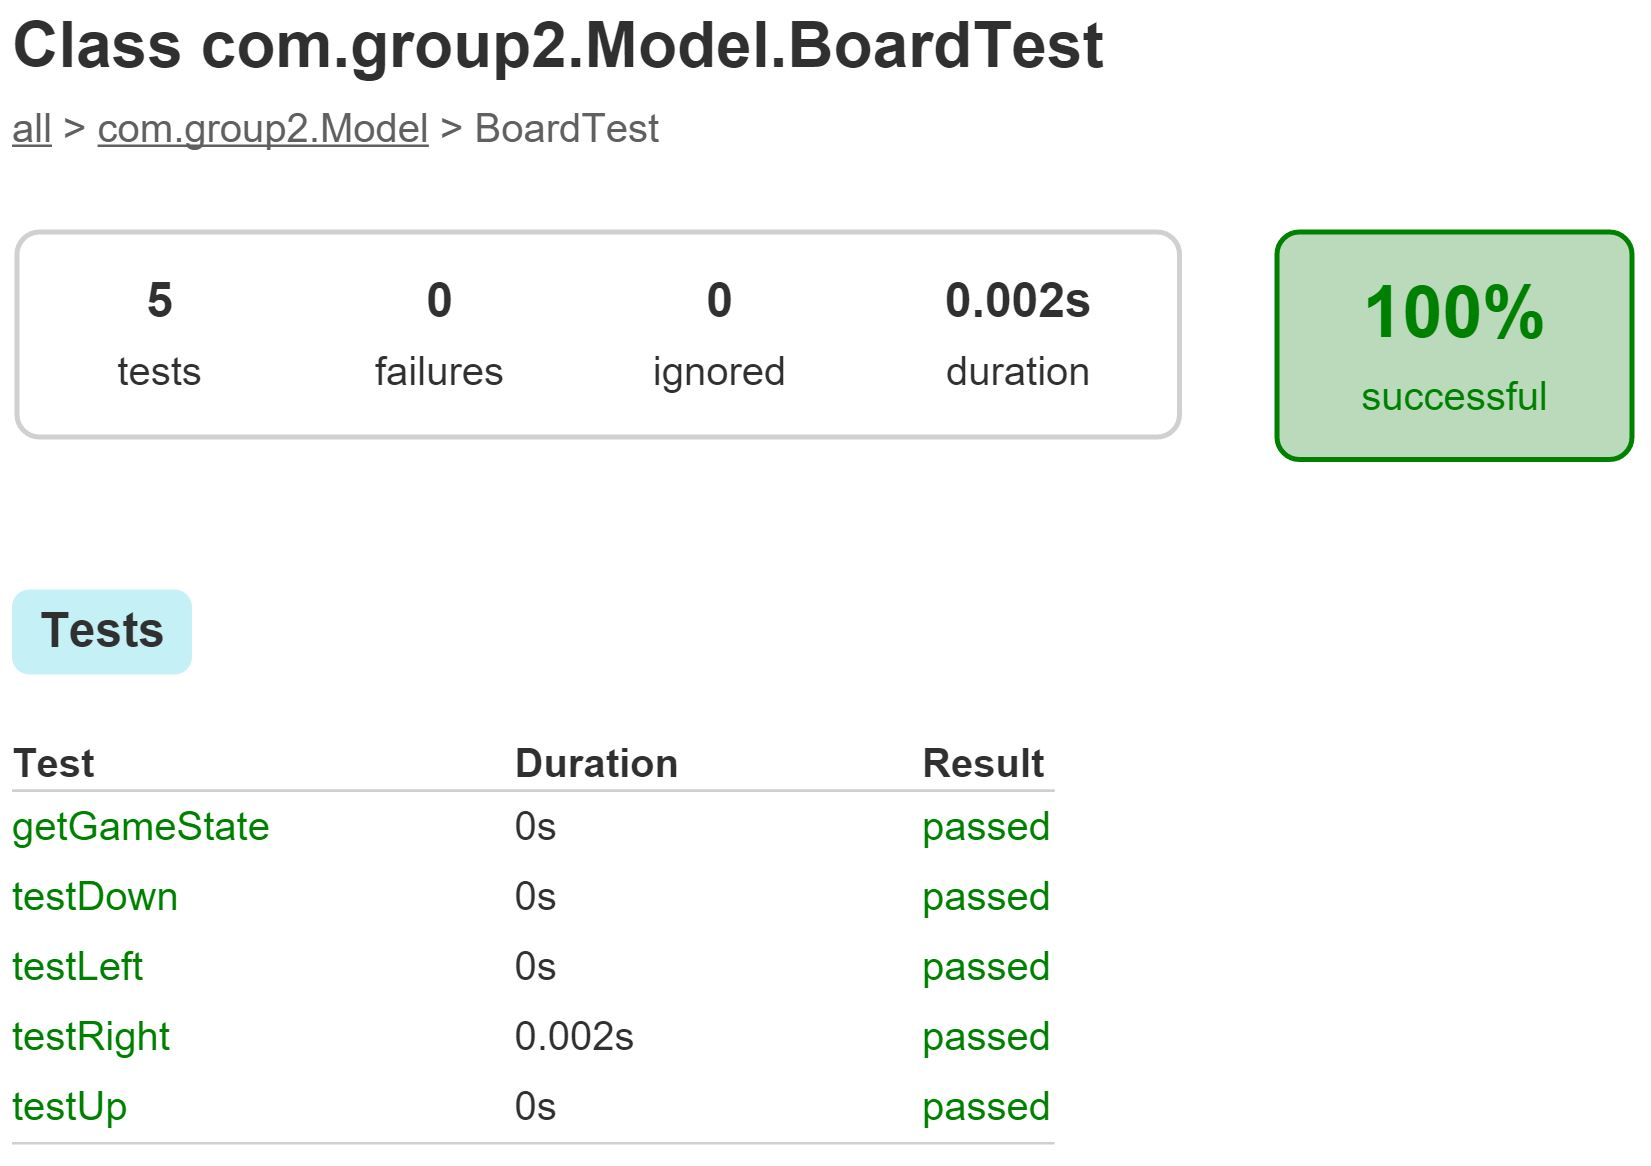
\includegraphics[width = 14cm]{JUnit_Test_Results}
	\caption{JUnit Test Results}
	\label{JUnit Test Results}
\end{figure}

\section{Non-Functional Qualities Testing}
\subsection{Usability}
\subsubsection{GUI}
	Testing the ease of use will be done through manual testing. It will be done by getting a set of users that have no background in computer science or any related fields, and getting feedback from them about the interface and how easy the game was to play. 
	\par The feedback from the users will be obtained through a questionnaire in which the questions are based on how easy the GUI and game, was to understand and use. The users will then rate their satisfaction on a scale of 1 to 5, where 5 is being completely satisfied and 1 is being completely unsatisfied. A copy of the questionnaire can be found in the Appendix.
	\par The results of the questionnaires will then be processed to give an average result/satisfaction rate on usability. This average will be compared to a usability criteria that is organized as follows:
\



\end{document}
